\documentclass[12pt, a4paper]{article}

\usepackage[utf8]{inputenc}
\usepackage[T1]{fontenc}
\usepackage[brazil]{babel}
\usepackage{geometry}
\geometry{a4paper, margin=3cm}
\usepackage{graphicx}
\usepackage{amsmath}
\usepackage{booktabs}
\usepackage{longtable}
\usepackage{hyperref}
\usepackage{cite}
\usepackage{xcolor}

\graphicspath{{./}{./images/}}

\hypersetup{
    colorlinks=true,
    linkcolor=blue,
    filecolor=magenta,
    urlcolor=cyan,
    citecolor=blue,
}

\title{
    \vspace{-1.5cm}
    \textbf{Sistema Automatizado de Limpeza e Arrefecimento de Painéis Fotovoltaicos (ASCM):\\
    Projeto, Implementação e Metodologia de Validação}
}

\author{
    César Kerber \\
    Lucas Ekroth \\
    Paulo Rangel \\
    \vspace{0.2cm}
    \small Curso de Engenharia de Controle e Automação \\
    \small Instituto Federal de Educação, Ciência e Tecnologia de São Paulo (IFSP) \\
    \small Câmpus São José dos Campos \\
    \small Orientador: Prof. Valdeci Donizete Gonçalves
}

\date{\today}

\begin{document}

\maketitle

\begin{abstract}
\noindent A eficiência de sistemas solares fotovoltaicos é severamente afetada por fatores ambientais externos, sendo o acúmulo de sujeira (\textit{soiling}) e o superaquecimento das células os dois principais fatores de perda de geração. Este trabalho apresenta o desenvolvimento completo de um protótipo de Sistema Automatizado de Limpeza e Arrefecimento de Painéis Fotovoltaicos (\textit{Automated Self-Cleaning and Cooling Mechanism} - ASCM), cobrindo desde o referencial teórico e o projeto mecânico em CAD até a arquitetura de software completa (firmware, backend e dashboard) e a metodologia experimental de validação. O sistema realiza a limpeza mecânica por meio de aspersão de água combinada com um rodo motorizado, e o resfriamento evaporativo por meio do acionamento de uma mini-bomba hidráulica. A lógica de controle é baseada em microcontrolador Arduino Uno rodando o protocolo Telemetrix, integrado a um backend em Python (FastAPI) responsável pela automação, persistência de dados e integração com serviços meteorológicos externos, e a um dashboard em Streamlit para monitoramento e controle manual em tempo real. O acionamento da limpeza é guiado de forma inteligente pela comparação diferencial de potência entre um painel principal e um painel de referência mantido sujo. Este documento detalha, em profundidade, cada subsistema do ASCM — eletrônica, mecânica, firmware, API REST e interface de usuário — além de estabelecer a metodologia para os ensaios de curto e longo prazo que validarão a remoção de sujidade induzida, a recuperação de eficiência e o ganho térmico do protótipo completo.
\end{abstract}

\textbf{Palavras-chave:} Energia Solar Fotovoltaica. Soiling. Arrefecimento Térmico. Automação. Arduino. FastAPI. Streamlit.

\newpage
\tableofcontents
\newpage

\section{Introdução}

\subsection{Contextualização}

A transição energética global em direção a fontes renováveis tem posicionado a energia solar fotovoltaica como um dos pilares fundamentais da matriz elétrica de diversos países. Segundo relatórios da organização de estudos energéticos \textit{Ember} \cite{ember_brazil_2024, ember_eu_2026}, o Brasil alcançou a marca histórica em que a geração eólica e solar fotovoltaica combinadas ultrapassam um terço da eletricidade produzida no país \cite{ember_brazil_2024}, conforme ilustrado na Figura \ref{fig:grafico_ember}. Paralelamente, na União Europeia, as fontes renováveis atingiram cerca de 30\% da matriz elétrica \cite{ember_eu_2026}. Com o crescimento exponencial da capacidade instalada, torna-se crítico assegurar que esses ativos operem com o máximo aproveitamento energético possível, uma vez que perdas percentuais pequenas, quando multiplicadas pela escala de gigawatts instalados, representam quantidades significativas de energia não gerada.

\begin{figure}[htbp]
    \centering
    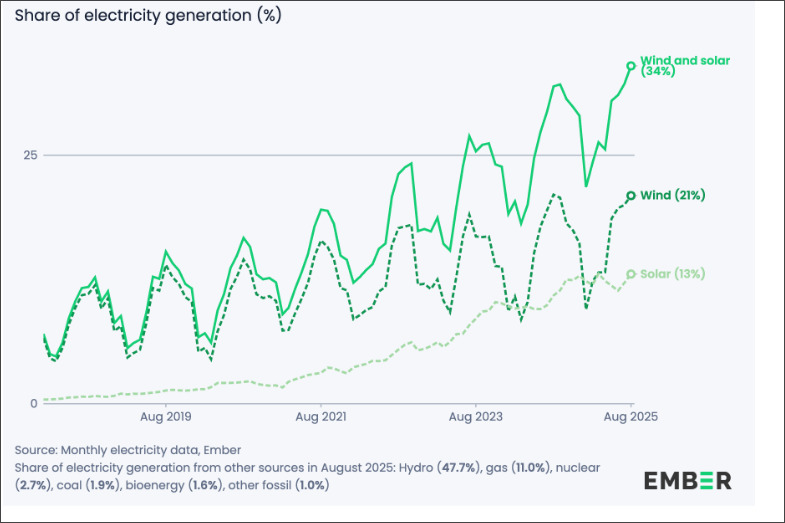
\includegraphics[width=0.65\textwidth]{grafico_ember.png}
    \caption{Geração elétrica renovável no Brasil, evidenciando o crescimento de eólica e solar.}
    \label{fig:grafico_ember}
    \centerline{\small Fonte: Adaptado de Ember (2024).}
\end{figure}

Apesar dos avanços tecnológicos nos materiais semicondutores, a eficiência operacional de um módulo fotovoltaico é drasticamente degradada por variáveis externas em campo. O primeiro fator crítico é o acúmulo de poeira, pólen, dejetos e poluentes suspensos no ar na superfície de vidro do painel, fenômeno conhecido na literatura como \textit{soiling} \cite{qi2025}. A poeira depositada obstrui a radiação solar direta que penetra nas junções p-n, diminuindo a corrente gerada. Estudos apontam que o acúmulo contínuo de poeira pode reduzir a eficiência do painel em até 7,84\% por semana em locais de alta taxa de deposição, podendo ultrapassar 50\% de perda total em períodos de seca prolongada sem intervenção humana ou precipitações pluviométricas de volume adequado \cite{qi2025}. O impacto negativo do acúmulo de sujidade na potência máxima de saída das células fotovoltaicas está quantificado graficamente na Figura \ref{fig:grafico_soiling}.

\begin{figure}[htbp]
    \centering
    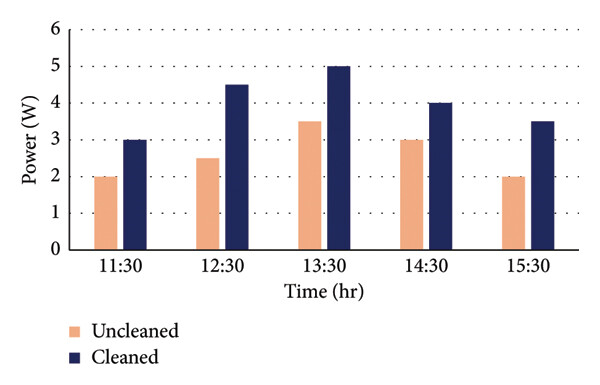
\includegraphics[width=0.55\textwidth]{grafico_soiling.jpg}
    \caption{Gráfico representativo das perdas na potência de saída em função da deposição de poeira ao longo de períodos secos.}
    \label{fig:grafico_soiling}
    \centerline{\small Fonte: Adaptado de Qi et al. (2025).}
\end{figure}

O segundo fator crítico relaciona-se ao coeficiente de temperatura do silício. O aquecimento natural do painel solar devido à radiação térmica eleva a temperatura de operação muito acima dos 25$^\circ$C padronizados em laboratório. Para cada grau Celsius acrescido à superfície, a potência máxima de saída do painel decresce linearmente entre 0,5\% e 0,6\% \cite{geetha2024}. A deposição de poeira agrava este quadro por atuar como isolante térmico local, mantendo o calor aprisionado sob a camada de sujeira e acelerando a degradação e o envelhecimento do módulo.

\subsection{Justificativa}

Diante desse cenário, soluções de baixo custo que combinem limpeza automática e arrefecimento ativo apresentam alto potencial técnico e econômico, sobretudo para instalações de pequeno e médio porte (residenciais e pequenos comércios), onde soluções industriais de limpeza robotizada são financeiramente inviáveis. A escolha por uma arquitetura baseada em componentes comerciais de prateleira (COTS), microcontrolador de baixo custo e software livre justifica-se pela necessidade de reprodutibilidade acadêmica e pela possibilidade de escalar o sistema para redes de múltiplos painéis sem custos proibitivos de licenciamento ou hardware proprietário.

\subsection{Objetivos}

\subsubsection{Objetivo Geral}
Desenvolver e validar um protótipo funcional de sistema automatizado de limpeza e arrefecimento de painéis fotovoltaicos (ASCM), capaz de detectar autonomamente a perda de eficiência por \textit{soiling} e por superaquecimento, e reagir com ciclos de limpeza mecânica e resfriamento evaporativo.

\subsubsection{Objetivos Específicos}
\begin{itemize}
    \item Projetar e fabricar, por manufatura aditiva (impressão 3D), o mecanismo eletromecânico de translação do rodo de limpeza;
    \item Especificar e integrar o hardware eletrônico de sensoriamento (potência, temperatura, luminosidade e fins de curso) e atuação (motor DC e bomba hidráulica);
    \item Desenvolver um firmware baseado no protocolo Telemetrix que dispense a necessidade de recompilação para alterações na lógica de controle;
    \item Implementar um backend em Python (FastAPI) responsável pela automação, persistência de telemetria e integração com serviços meteorológicos externos;
    \item Implementar um dashboard web (Streamlit) para monitoramento em tempo real e controle manual de emergência;
    \item Estabelecer e documentar a metodologia de ensaios de curto prazo (ambiente controlado) e de longo prazo (campo) para validação quantitativa do sistema.
\end{itemize}

\subsection{Estrutura do Trabalho}

Este documento está organizado da seguinte forma: a Seção \ref{sec:referencial} apresenta o referencial teórico sobre soiling, arrefecimento térmico e trabalhos correlatos. A Seção \ref{sec:metodologia} detalha a arquitetura completa do sistema — hardware, mecânica, firmware, backend, dashboard e estratégia de controle. A Seção \ref{sec:resultados} apresenta os resultados preliminares de validação de software e a metodologia projetada para os ensaios físicos. Por fim, a Seção \ref{sec:conclusao} apresenta as considerações finais e os próximos passos do projeto.

\section{Referencial Teórico e Estado da Arte}
\label{sec:referencial}

\subsection{Mecanismos de Limpeza Ativa e Passiva}

A literatura científica classifica os métodos de higienização de painéis fotovoltaicos em duas principais categorias:
\begin{itemize}
    \item \textbf{Métodos Passivos (Revestimentos):} Utilizam nanotecnologia aplicada à superfície do vidro para formar películas super-hidrofóbicas. Esses revestimentos diminuem o ângulo de contato da água e reduzem as forças de adesão de Van der Waals das partículas de poeira \cite{qi2025}. Embora promissores, apresentam custo elevado de aplicação e vida útil curta sob intempéries e abrasão mecânica.
    \item \textbf{Métodos Ativos (Mecânicos e Pneumáticos):} Compreendem sistemas que despendem energia para a remoção da poeira. Os robôs autônomos utilizam esteiras e escovas rotativas para transladar entre painéis. Entretanto, sua complexidade e custo são proibitivos para instalações de pequeno e médio porte. Os sistemas de aspersão com bicos aspersores combinados a rodos motorizados (\textit{wipers}) destacam-se pelo equilíbrio entre custo de instalação e alta eficácia. Estudos práticos realizados por Geetha et al. \cite{geetha2024} indicaram um aumento real de 14,81\% na potência de saída utilizando esta abordagem de aspersão com limpeza mecânica controlada por microcontrolador.
\end{itemize}

\subsection{O Fenômeno de Cristalização de Sujeira (\textit{Dust Scaling})}

Estudos de Qi et al. \cite{qi2025} apontam que a interação da poeira seca com a umidade do ar (como o orvalho matinal) é responsável pelo fenômeno de \textit{dust scaling} ou formação de crosta rígida (\textit{hard scale}). Quando a umidade relativa situa-se na faixa entre 40\% e 80\%, formam-se pontes de água microscópicas por capilaridade entre as partículas de poeira e o vidro. Após o nascer do sol e subsequente evaporação da água, sais minerais solúveis cristalizam-se, cimentando a sujeira na superfície. A remoção de tal camada torna-se inviável por meio de métodos puramente a seco (como sopro de ar ou escovação seca simples), exigindo o uso controlado de água como solvente mecânico aliado ao atrito de um rodo.

\subsection{Arrefecimento Térmico Ativo}

Sistemas automáticos de limpeza e arrefecimento ativo demonstram-se soluções promissoras e de baixo custo para mitigar as perdas conjuntas de soiling e temperatura \cite{derakhshandeh2021}, inclusive com estratégias de controle dinâmicas baseadas nas condições climáticas em tempo real, como o acompanhamento de previsão de chuva e temperatura ambiente para evitar acionamentos desnecessários \cite{mendis2026}. O resfriamento evaporativo, obtido pela aspersão de uma fina lâmina d'água sobre o vidro do painel, retira calor da superfície tanto pela troca convectiva direta com a água quanto pela evaporação subsequente, sendo uma técnica de baixo custo energético comparada a sistemas de refrigeração ativa (Peltier ou compressores).

\subsection{Gestão Hídrica}

Um desafio frequente na higienização por aspersão é o consumo de água, elemento que pode impactar negativamente a sustentabilidade ecológica e econômica do projeto. Autores como Cavalcante et al. \cite{cavalcante2016} propõem a implementação de captação de água pluvial conjugada a filtros físicos de sedimentação e filtragem de partículas grossas e finas no reservatório do próprio sistema fotovoltaico. Tal abordagem reduz o consumo líquido de água potável da rede de distribuição a níveis próximos de zero, viabilizando o sistema para regiões semiáridas ou remotas.

\subsection{Síntese Comparativa dos Trabalhos Correlatos}

A Tabela \ref{tab:trabalhos_correlatos} sintetiza as principais abordagens discutidas na literatura consultada, contrastando-as com a proposta do ASCM em termos de mecanismo de acionamento, uso de água e integração com sensoriamento inteligente.

\begin{table}[htbp]
    \centering
    \caption{Comparativo entre abordagens de limpeza/arrefecimento na literatura e o ASCM.}
    \label{tab:trabalhos_correlatos}
    \begin{tabular}{p{2.6cm}p{3.6cm}p{2.2cm}p{4.4cm}}
    \toprule
    \textbf{Referência} & \textbf{Mecanismo} & \textbf{Uso de Água} & \textbf{Controle} \\
    \midrule
    Geetha et al. \cite{geetha2024} & Aspersão + limpeza mecânica & Sim & Microcontrolador, acionamento simples \\
    Derakhshandeh et al. \cite{derakhshandeh2021} & Revisão de sistemas automáticos diversos & Variável & Diversos, sem padrão único \\
    Mendis et al. \cite{mendis2026} & Rastreamento solar dual-eixo + autolimpeza & Não especificado & Reativo às condições climáticas em tempo real \\
    Cavalcante et al. \cite{cavalcante2016} & Aspersão com reaproveitamento hídrico & Sim (pluvial) & Manual/temporizado \\
    \textbf{ASCM (este trabalho)} & Aspersão + rodo motorizado (\textit{gear-rack}) & Sim (dosada) & Diferencial de potência entre painéis + API de clima \\
    \bottomrule
    \end{tabular}
\end{table}

Observa-se que a maioria dos trabalhos correlatos aciona a limpeza de forma temporizada ou puramente reativa à temperatura, ao passo que o ASCM soma dois critérios independentes (perda diferencial de potência e previsão de chuva) para decidir o acionamento, reduzindo o desperdício de água em ciclos desnecessários.

\section{Materiais e Métodos}
\label{sec:metodologia}

O protótipo do sistema ASCM foi desenvolvido utilizando componentes comerciais de prateleira (COTS - \textit{Commercial Off-The-Shelf}) visando manter a replicabilidade e o baixo custo de fabricação. A arquitetura divide-se em: Hardware Eletrônico, Projeto Mecânico, Firmware, Backend, Dashboard e Estratégia de Controle.

\subsection{Visão Geral da Arquitetura}

A Figura \ref{fig:fluxograma_controle} (Seção \ref{sec:estrategia-controle}) resume o funcionamento macro do sistema: sensores conectados ao Arduino Uno alimentam, via protocolo serial Telemetrix, um backend Python que centraliza a lógica de decisão, persiste os dados e expõe uma API REST consumida tanto pelo laço de automação interno quanto pelo dashboard Streamlit usado pelo operador humano.

\subsection{Especificação e Arquitetura de Hardware}

O hardware eletrônico está centrado no microcontrolador Arduino Uno R3. A Tabela \ref{tab:bom} apresenta a lista de materiais (BOM) do protótipo, e a Tabela \ref{tab:pinout} detalha o mapeamento de pinos utilizado, ambos documentados de forma exaustiva no Guia de Hardware do projeto \cite{electronics_guide}.

\begin{table}[htbp]
    \centering
    \caption{Lista de materiais (BOM) do protótipo ASCM.}
    \label{tab:bom}
    \begin{tabular}{p{3.2cm}p{1.2cm}p{4.0cm}p{4.4cm}}
    \toprule
    \textbf{Item} & \textbf{Qtd.} & \textbf{Descrição} & \textbf{Função} \\
    \midrule
    Microcontrolador & 1 & Arduino Uno R3 & Interface de I/O (firmware Telemetrix) \\
    Driver de Motor & 1 & Ponte H L298N & Controle do motor de movimentação (\textit{wiper}) \\
    Motor DC & 1 & Motor 5V com redução & Movimentação da escova/rodo \\
    Bomba d'água & 1 & Mini-bomba submersível 5V & Aspersão e arrefecimento \\
    Sensores de Potência & 2 & Módulo INA219 ($I^2C$) & Monitoramento de V/I do painel principal e de referência \\
    Sensores Fim de Curso & 2 & Micro-switch (NF/NA) & Limitação física do curso do rodo \\
    Sensor de Temperatura & 1 & Termopar/LM35 & Monitoramento térmico da superfície \\
    Sensor de Luz & 1 & LDR & Medição de irradiância relativa \\
    Resistor de Carga & 2 & 33 $\Omega$ ($\geq$ 1,5W) & Carga para medição de potência dos painéis \\
    Resistor LDR & 1 & 10 k$\Omega$ & Divisor de tensão do LDR \\
    Painel Solar & 2 & Módulos fotovoltaicos & Geração de energia e referência de sujeira \\
    \bottomrule
    \end{tabular}
\end{table}

\begin{table}[htbp]
    \centering
    \caption{Mapeamento de pinos (\textit{pinout}) do Arduino Uno no protótipo ASCM.}
    \label{tab:pinout}
    \begin{tabular}{p{4.2cm}p{1.6cm}p{2.0cm}p{5.0cm}}
    \toprule
    \textbf{Componente} & \textbf{Pino} & \textbf{Tipo} & \textbf{Descrição} \\
    \midrule
    Ponte H (ENA) & 11 & PWM & Velocidade do motor (\textit{wiper}) \\
    Ponte H (IN1) & 9 & Digital & Direção do motor (\textit{wiper}) \\
    Ponte H (IN2) & 10 & Digital & Direção do motor (\textit{wiper}) \\
    Ponte H (ENB) & 6 & PWM & Velocidade/fluxo da bomba \\
    Ponte H (IN3) & 7 & Digital & Ativação da bomba \\
    Ponte H (IN4) & 8 & Digital & Ativação da bomba \\
    Fim de Curso (Home) & 2 & Digital & Sensor de posição inicial \\
    Fim de Curso (End) & 3 & Digital & Sensor de posição final \\
    LDR & A0 & Analógico & Leitura de luminosidade \\
    Temperatura & A1 & Analógico & Leitura de temperatura da superfície \\
    INA219 Principal & A4/A5 & $I^2C$ (0x40) & Painel monitorado/limpo pelo sistema \\
    INA219 Referência & A4/A5 & $I^2C$ (0x41) & Painel de referência (sujeira natural) \\
    \bottomrule
    \end{tabular}
\end{table}

O sensor principal (endereço $I^2C$ $0x40$) monitora o painel limpo pelo sistema, enquanto o segundo sensor (endereço $0x41$, obtido por meio de uma ponte de solda no pino de endereço A0 do módulo) monitora o painel de referência, mantido propositalmente sujo. Ambas as saídas dos painéis são aplicadas sobre resistores de carga de 33 $\Omega$ e potência mínima de 1,5W para simular o consumo constante de carga. A alimentação de potência da Ponte H é provida externamente por uma fonte CC de 5V dedicada a motores e bomba, compartilhando a mesma referência de terra (GND) com o Arduino. O diagrama de conexões elétricas está ilustrado na Figura \ref{fig:diagrama_eletronica}.

\begin{figure}[htbp]
    \centering
    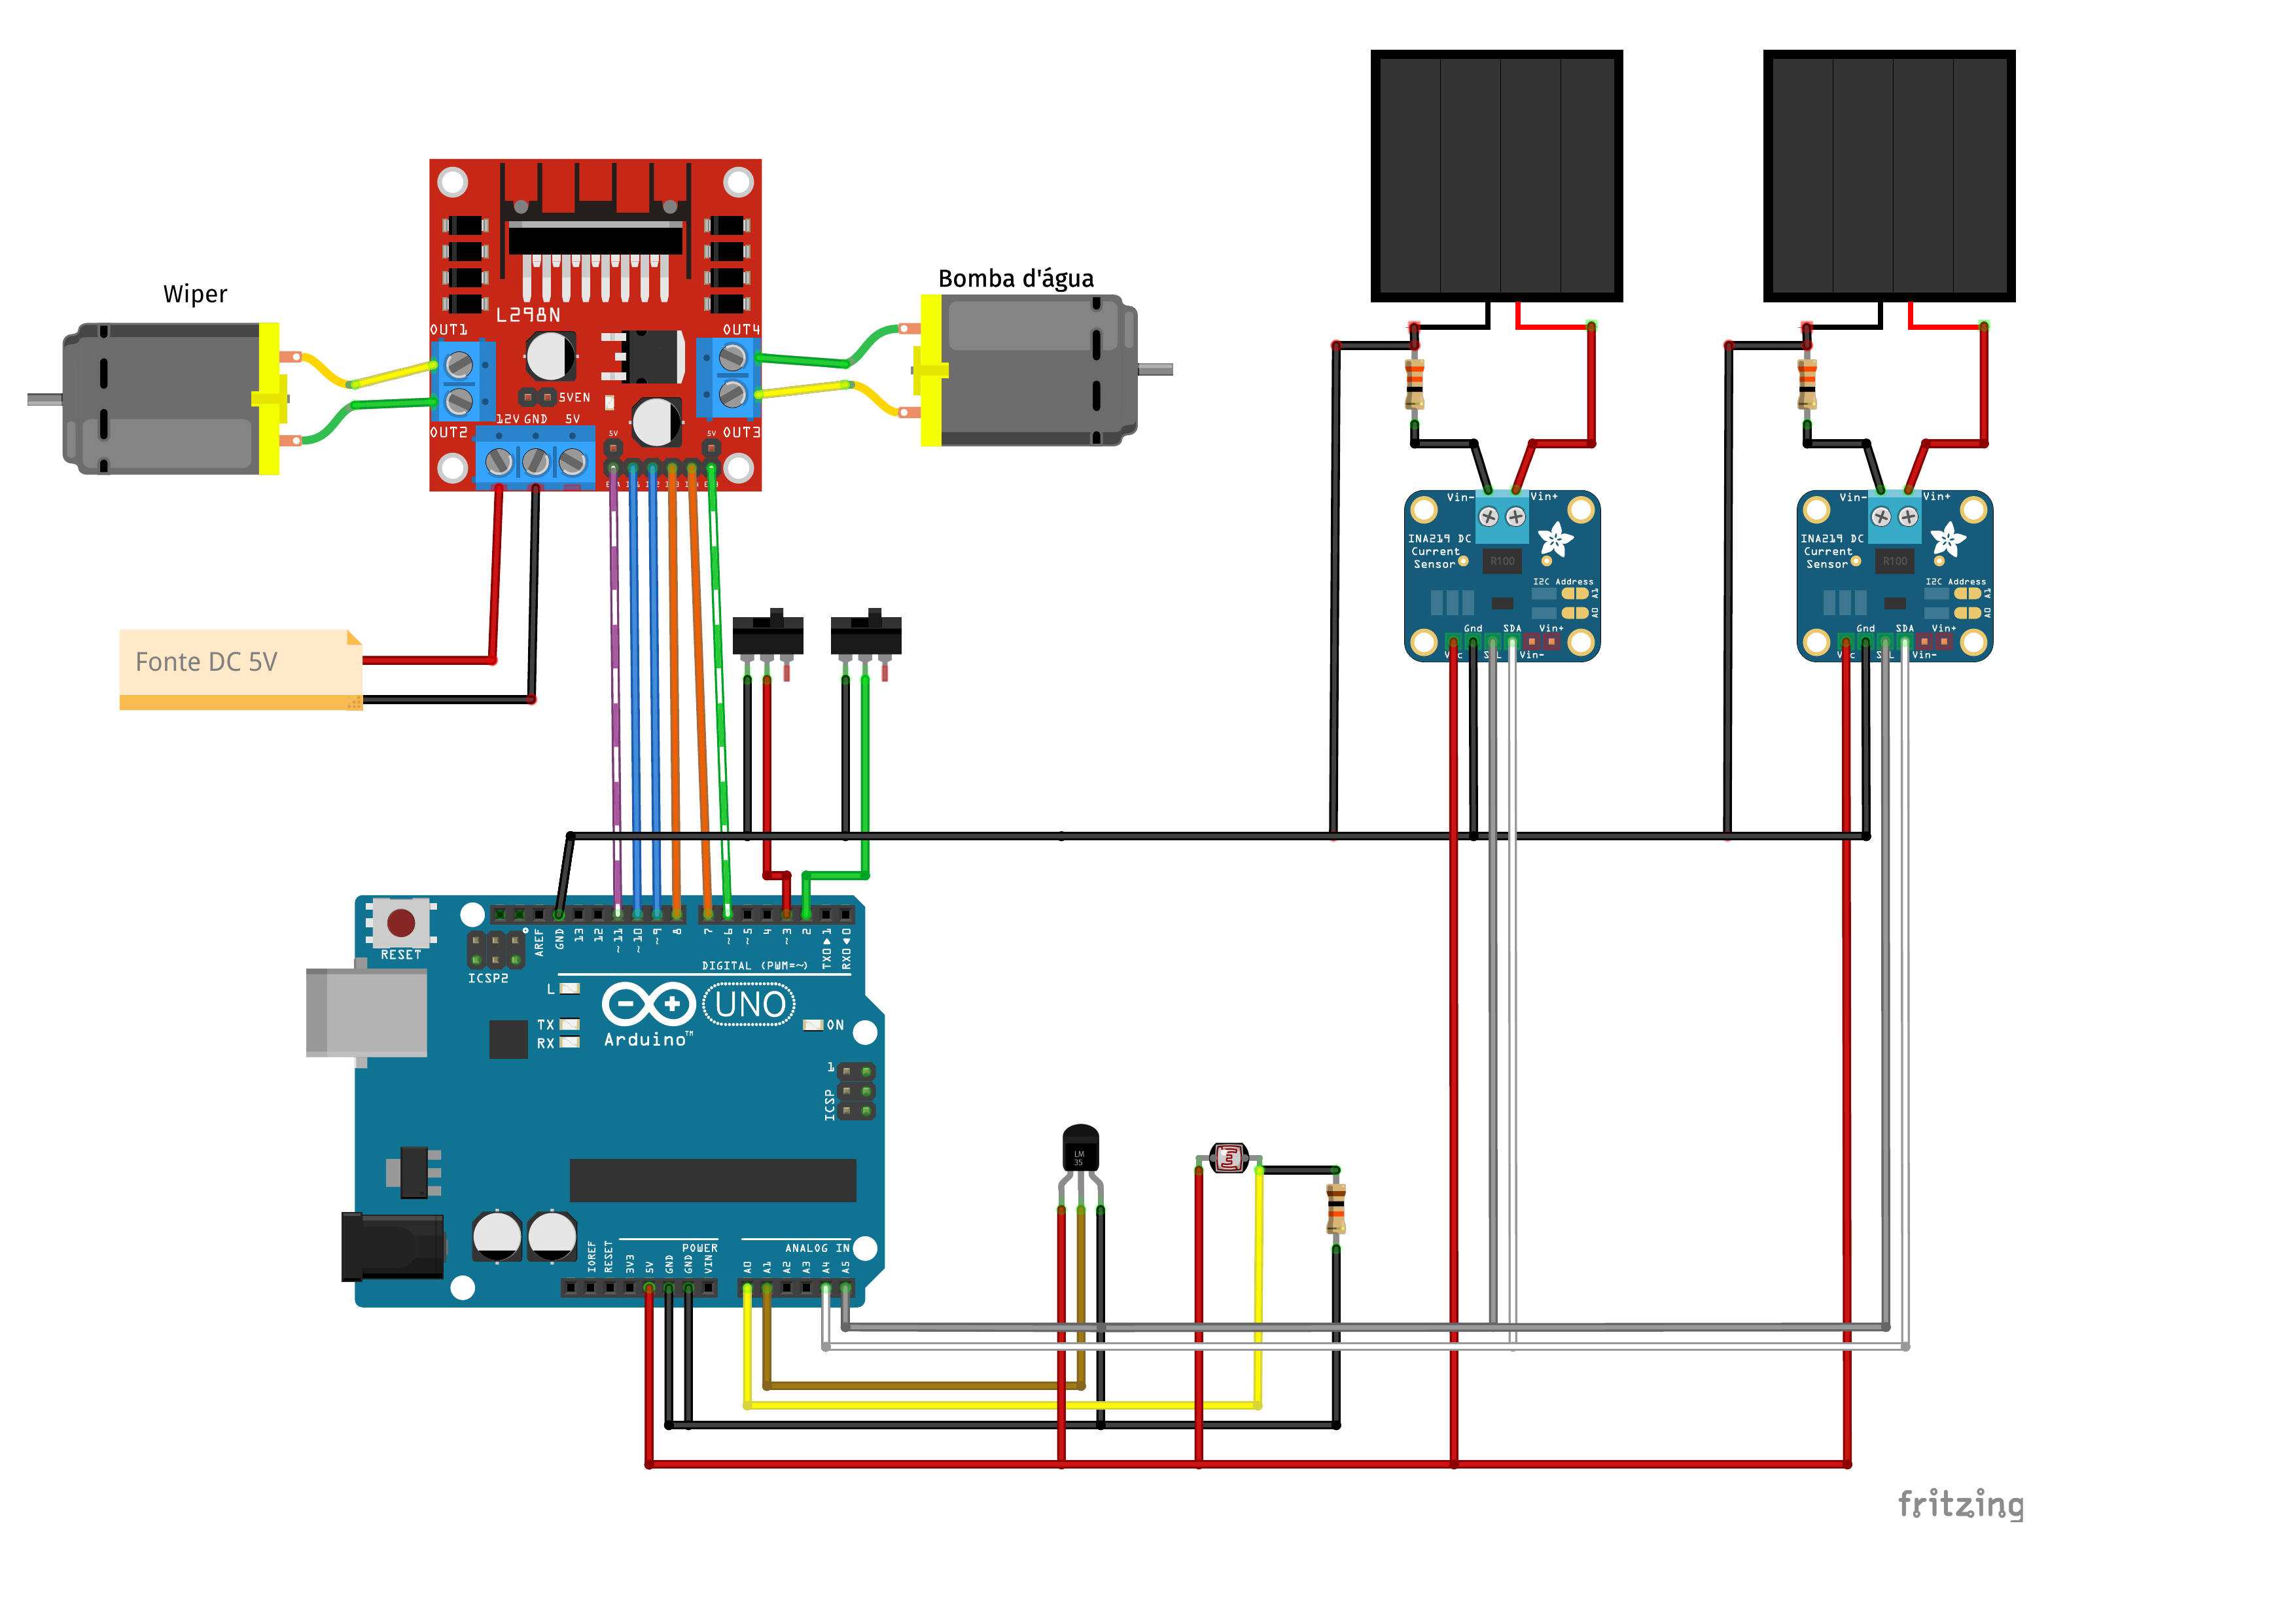
\includegraphics[width=0.7\textwidth]{diagrama_eletronica.png}
    \caption{Diagrama de conexões elétricas e esquemático de montagem física dos componentes eletrônicos do ASCM.}
    \label{fig:diagrama_eletronica}
    \centerline{\small Fonte: Elaborado pelos autores.}
\end{figure}

\subsection{Projeto Mecânico e Modelagem 3D}

O design estrutural e o mecanismo de movimentação linear do ASCM foram totalmente modelados utilizando o software de CAD tridimensional Autodesk Inventor, visando a prototipagem rápida através da fabricação por manufatura aditiva (impressão 3D por deposição de material fundido - FDM). O design mecânico compreende a modelagem dos seguintes componentes principais:
\begin{itemize}
    \item \textbf{Mecanismo de Transmissão por Pinhão e Cremalheira (\textit{Gear and Rack}):} Para evitar deslizamentos mecânicos comuns em transmissões por polia e correia sob condições de umidade e exposição direta a respingos de água, o sistema adota um mecanismo de pinhão e cremalheira. A cremalheira (\textit{Gear-Rack}) é fixada ao longo do trilho de deslizamento, e o pinhão (\textit{Gear} acoplado ao eixo do motor DC) engrena diretamente na cremalheira para guiar a translação suave do rodo.
    \item \textbf{Suporte do Rodo (\textit{Wiper Support}):} Peça personalizada que aloja o motor de tração com redução e fixa a haste do rodo de silicone contra a superfície do vidro do painel principal, garantindo uma pressão de contato uniforme para a varredura da poeira.
    \item \textbf{Suporte de Aspersão (\textit{Sprinkler Support}):} Fixadores posicionados no topo do painel que sustentam a tubulação hidráulica e os bicos aspersores orientados em ângulo que maximiza a área de cobertura da lâmina d'água na superfície.
    \item \textbf{Suportes dos Painéis (\textit{Panel Support}):} Peças de interface que prendem os módulos fotovoltaicos de forma rígida à estrutura de suporte principal.
\end{itemize}
A modelagem em CAD de todas as peças foi exportada em formato STL para fabricação por manufatura aditiva. Para a confecção do protótipo físico de teste, utilizou-se filamento de PLA (Ácido Polilático) pela facilidade de prototipagem rápida e baixo custo, embora materiais como PETG ou ABS possam ser aplicados em versões finais expostas a intempéries contínuas caso o equipamento de impressão ofereça suporte a tais polímeros. A vista explodida da montagem, evidenciando o encaixe entre a cremalheira linear, o pinhão e o suporte do rodo motorizado, está ilustrada na Figura \ref{fig:vista_explodida}.

\begin{figure}[htbp]
    \centering
    \IfFileExists{images/vista_explodida.png}{%
        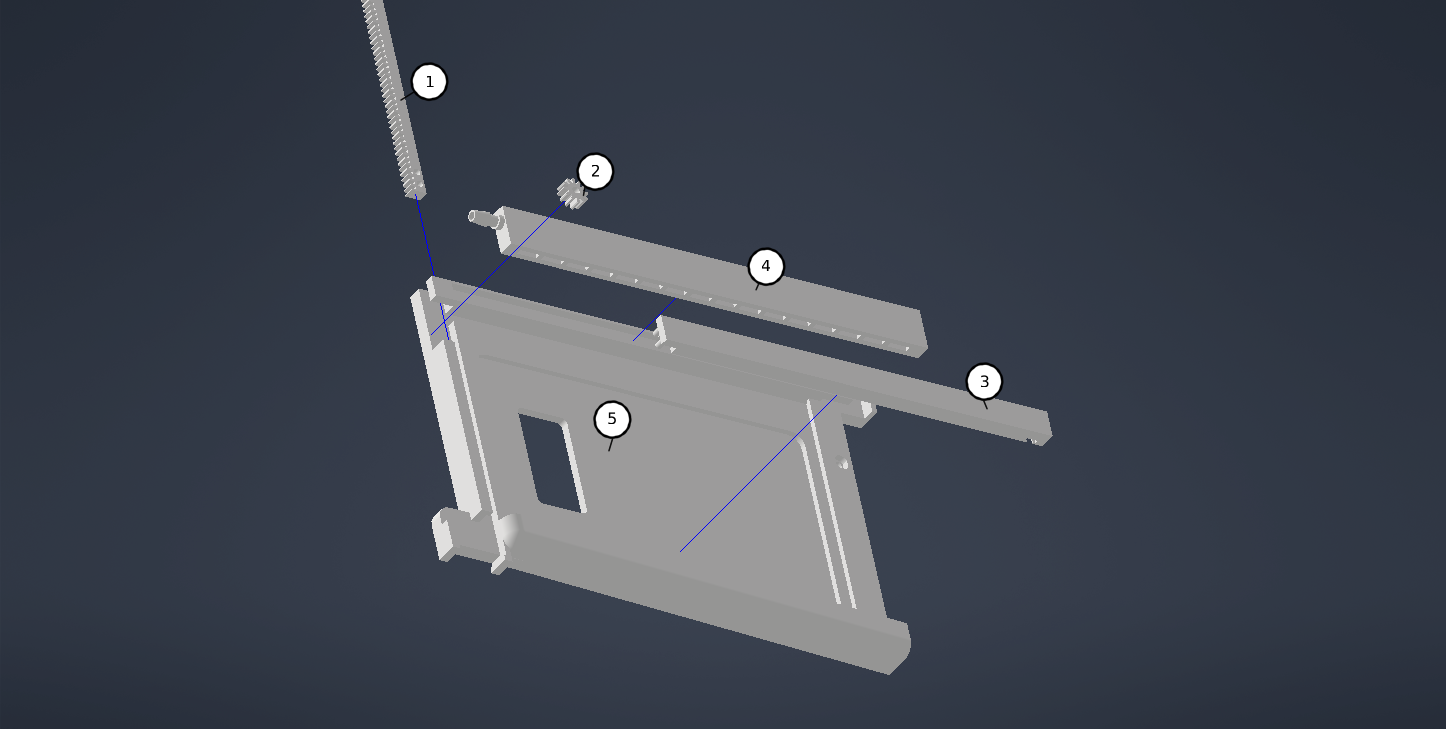
\includegraphics[width=0.9\textwidth]{vista_explodida.png}%
    }{%
        \fbox{\parbox[c][6cm][c]{0.9\textwidth}{\centering\textit{Vista explodida da montagem (pendente)}}}%
    }
    \caption{Vista explodida da montagem do mecanismo de translação do ASCM: (1) Cremalheira (\textit{Gear-Rack}); (2) Pinhão (\textit{Gear}); (3) Suporte do Rodo (\textit{Wiper Support}); (4) Suporte de Aspersão (\textit{Sprinkler}); (5) Suporte dos Painéis (\textit{Panel Support}).}
    \label{fig:vista_explodida}
    \centerline{\small Fonte: Elaborado pelos autores.}
\end{figure}

\subsection{Arquitetura de Software}

Ao contrário de abordagens convencionais com firmware C/C++ estático compilado no Arduino, o ASCM adota a arquitetura \textbf{Telemetrix} \cite{telemetrix_ref, telemetrix_doc}. O Arduino Uno executa o sketch padrão \textit{Telemetrix4Arduino}, operando puramente como um dispositivo escravo de entrada e saída (servidor de I/O) que se comunica via porta serial com um computador hospedeiro. Toda a lógica de controle complexa, o tratamento matemático e os registros de log são implementados na linguagem Python no computador servidor, dividida em três camadas: firmware/driver de hardware, backend (API) e frontend (dashboard).

\subsubsection{Camada de Hardware (\texttt{HardwareManager})}

A classe \texttt{HardwareManager} encapsula toda a comunicação com o Arduino via Telemetrix. Na inicialização, ela configura os modos de pino (saídas digitais para a Ponte H, entradas digitais com \textit{pull-up} para os fins de curso, entradas analógicas para o LDR e o termopar, e o barramento $I^2C$ para os sensores INA219) e registra funções de \textit{callback} assíncronas para cada sensor. As leituras de temperatura e luminosidade passam por um filtro de média móvel com janela de 50 amostras (\texttt{\_temp\_history}, \texttt{\_lux\_history}) para atenuar o ruído inerente às leituras analógicas do LM35 e do LDR. A leitura de potência dos módulos INA219 é feita em duas etapas assíncronas (registrador de tensão de \textit{shunt}, para corrente, e registrador de tensão de barramento, para tensão), sendo a potência instantânea recalculada a cada atualização de tensão recebida.

Os métodos de atuação (\texttt{set\_pump}, \texttt{move\_wiper}, \texttt{stop\_wiper}) implementam trava de segurança por software: o método \texttt{move\_wiper} somente aciona o motor no sentido \textit{forward} se o fim de curso final (\texttt{limit\_end}) ainda não tiver sido atingido, e apenas no sentido \textit{backward} se o fim de curso inicial (\texttt{limit\_home}) ainda estiver aberto, evitando colisões mecânicas mesmo em caso de falha de lógica no nível do backend.

\subsubsection{Backend (FastAPI)}

O backend, implementado com o \textit{framework} FastAPI \cite{fastapi_doc}, expõe uma API REST responsável por três funções centrais: (i) leitura de telemetria em tempo real; (ii) execução de comandos manuais de atuadores; e (iii) execução do laço de automação assíncrono em segundo plano (\texttt{automation\_loop}), que roda a cada 60 segundos e é responsável por registrar a telemetria em disco, avaliar o critério de arrefecimento térmico e avaliar o critério de limpeza por \textit{soiling}. A Tabela \ref{tab:endpoints} documenta todos os \textit{endpoints} disponíveis na API.

\begin{table}[htbp]
    \centering
    \caption{Endpoints da API REST do backend ASCM (FastAPI).}
    \label{tab:endpoints}
    \begin{tabular}{p{1.4cm}p{3.2cm}p{7.2cm}}
    \toprule
    \textbf{Método} & \textbf{Rota} & \textbf{Descrição} \\
    \midrule
    GET & \texttt{/telemetry} & Retorna o estado completo dos sensores em cache (potência dos dois painéis, temperatura, luminosidade, fins de curso, estado da bomba/rodo e flag de limpeza ativa). \\
    GET & \texttt{/weather} & Consulta o serviço meteorológico externo (Open-Meteo) para a latitude/longitude configuradas e retorna temperatura ambiente, umidade, vento e indicação de chuva. \\
    POST & \texttt{/config/update} & Atualiza em tempo real os parâmetros de automação (latitude, longitude, limiar de sujeira, delta de temperatura, habilitação da automação). \\
    POST & \texttt{/cycle/cool} & Aciona manualmente a bomba em fluxo alto para arrefecimento imediato. \\
    POST & \texttt{/cycle/clean} & Dispara, como tarefa em segundo plano, o ciclo completo de limpeza (aspersão + varredura do rodo + retorno). Retorna erro HTTP 409 caso um ciclo já esteja em andamento. \\
    POST & \texttt{/actuators/pump} & Controle manual da bomba, recebendo o nível desejado (\texttt{high}, \texttt{low} ou \texttt{off}). \\
    GET & \texttt{/sensors/temperature} & Retorna isoladamente a temperatura atual da superfície do painel. \\
    GET & \texttt{/sensors/lux} & Retorna isoladamente a leitura de luminosidade relativa (LDR). \\
    GET & \texttt{/sensors/power} & Retorna as grandezas elétricas (tensão, corrente, potência) dos painéis principal e de referência. \\
    POST & \texttt{/actuators/motor} & Controle manual do motor do rodo, recebendo direção (\texttt{forward}/\texttt{backward}) e velocidade PWM opcional. \\
    POST & \texttt{/stop} & Parada de emergência: desliga a bomba e o motor do rodo imediatamente, independentemente do estado do laço de automação. \\
    \bottomrule
    \end{tabular}
\end{table}

O ciclo completo de limpeza, disparado por \texttt{/cycle/clean} ou automaticamente pelo laço de automação, é executado pela função \texttt{run\_full\_clean\_cycle}: a bomba é acionada em fluxo baixo por 2 segundos para umedecer e amolecer o \textit{hard scale}; em seguida o motor do rodo avança até atingir o fim de curso final (com um \textit{timeout} de segurança de 30 segundos contra travamentos mecânicos); o motor é parado por 1 segundo; o motor reverte o sentido até atingir o fim de curso inicial (também com \textit{timeout} de 30 segundos); e, por fim, a bomba e o motor são desligados, encerrando o ciclo.

\paragraph{Persistência e Serviços Auxiliares.} O módulo \texttt{CSVLogger} registra dois arquivos CSV independentes em disco: \texttt{telemetry\_history.csv} (uma linha por ciclo do laço de automação, contendo potência de ambos os painéis, temperatura, luminosidade e estado dos fins de curso) e \texttt{events\_history.csv} (registro cronológico de eventos discretos como início/fim de limpeza, acionamento de arrefecimento e paradas de emergência). O módulo \texttt{WeatherService} consulta a API pública Open-Meteo, sem necessidade de chave de autenticação, retornando temperatura ambiente, umidade relativa, velocidade do vento, pressão e um indicador booleano de chuva (derivado do campo de precipitação instantânea) e de previsão de chuva nas próximas três horas, usado para suprimir ciclos de limpeza que seriam naturalmente executados pela chuva.

\subsubsection{Frontend (Dashboard Streamlit)}

O dashboard, implementado com o \textit{framework} Streamlit \cite{streamlit_doc}, provê uma interface web para monitoramento instantâneo e controle manual do ASCM, consumindo diretamente os \textit{endpoints} da Tabela \ref{tab:endpoints} via requisições HTTP. A Figura \ref{fig:dashboard} apresenta o dashboard renderizado com dados de exemplo, evidenciando suas quatro regiões principais:

\begin{itemize}
    \item \textbf{Barra Lateral (Configurações e Status):} Permite ajustar em tempo real, via \texttt{/config/update}, a latitude/longitude usadas na consulta meteorológica, o limiar percentual de sujeira que dispara a limpeza e o delta de temperatura que dispara o arrefecimento, além de uma chave para habilitar/desabilitar a automação. Também exibe o status bruto dos sensores de fim de curso e um resumo das condições climáticas locais (condição, temperatura externa, vento e umidade), obtidos via \texttt{/telemetry} e \texttt{/weather}.
    \item \textbf{Cabeçalho de Métricas Instantâneas:} Exibe a temperatura do painel (com o delta em relação à temperatura ambiente), a luminosidade relativa e o estado da automação.
    \item \textbf{Comparativo de Geração:} Exibe lado a lado a potência do painel principal e do painel de referência, calculando em tempo real a perda percentual por \textit{soiling} ($\Delta \eta$) e emitindo um alerta visual quando essa perda ultrapassa o limiar configurado.
    \item \textbf{Comandos Manuais e Histórico:} Botões para disparar o ciclo completo de limpeza (\texttt{/cycle/clean}), o arrefecimento isolado (\texttt{/cycle/cool}), o retorno do rodo à posição \textit{home} e a parada de emergência (\texttt{/stop}), todos desabilitados durante um ciclo de limpeza já em andamento para evitar comandos conflitantes. Um gráfico de linha exibe o histórico recente de potência gerada por ambos os painéis.
\end{itemize}

\begin{figure}[htbp]
    \centering
    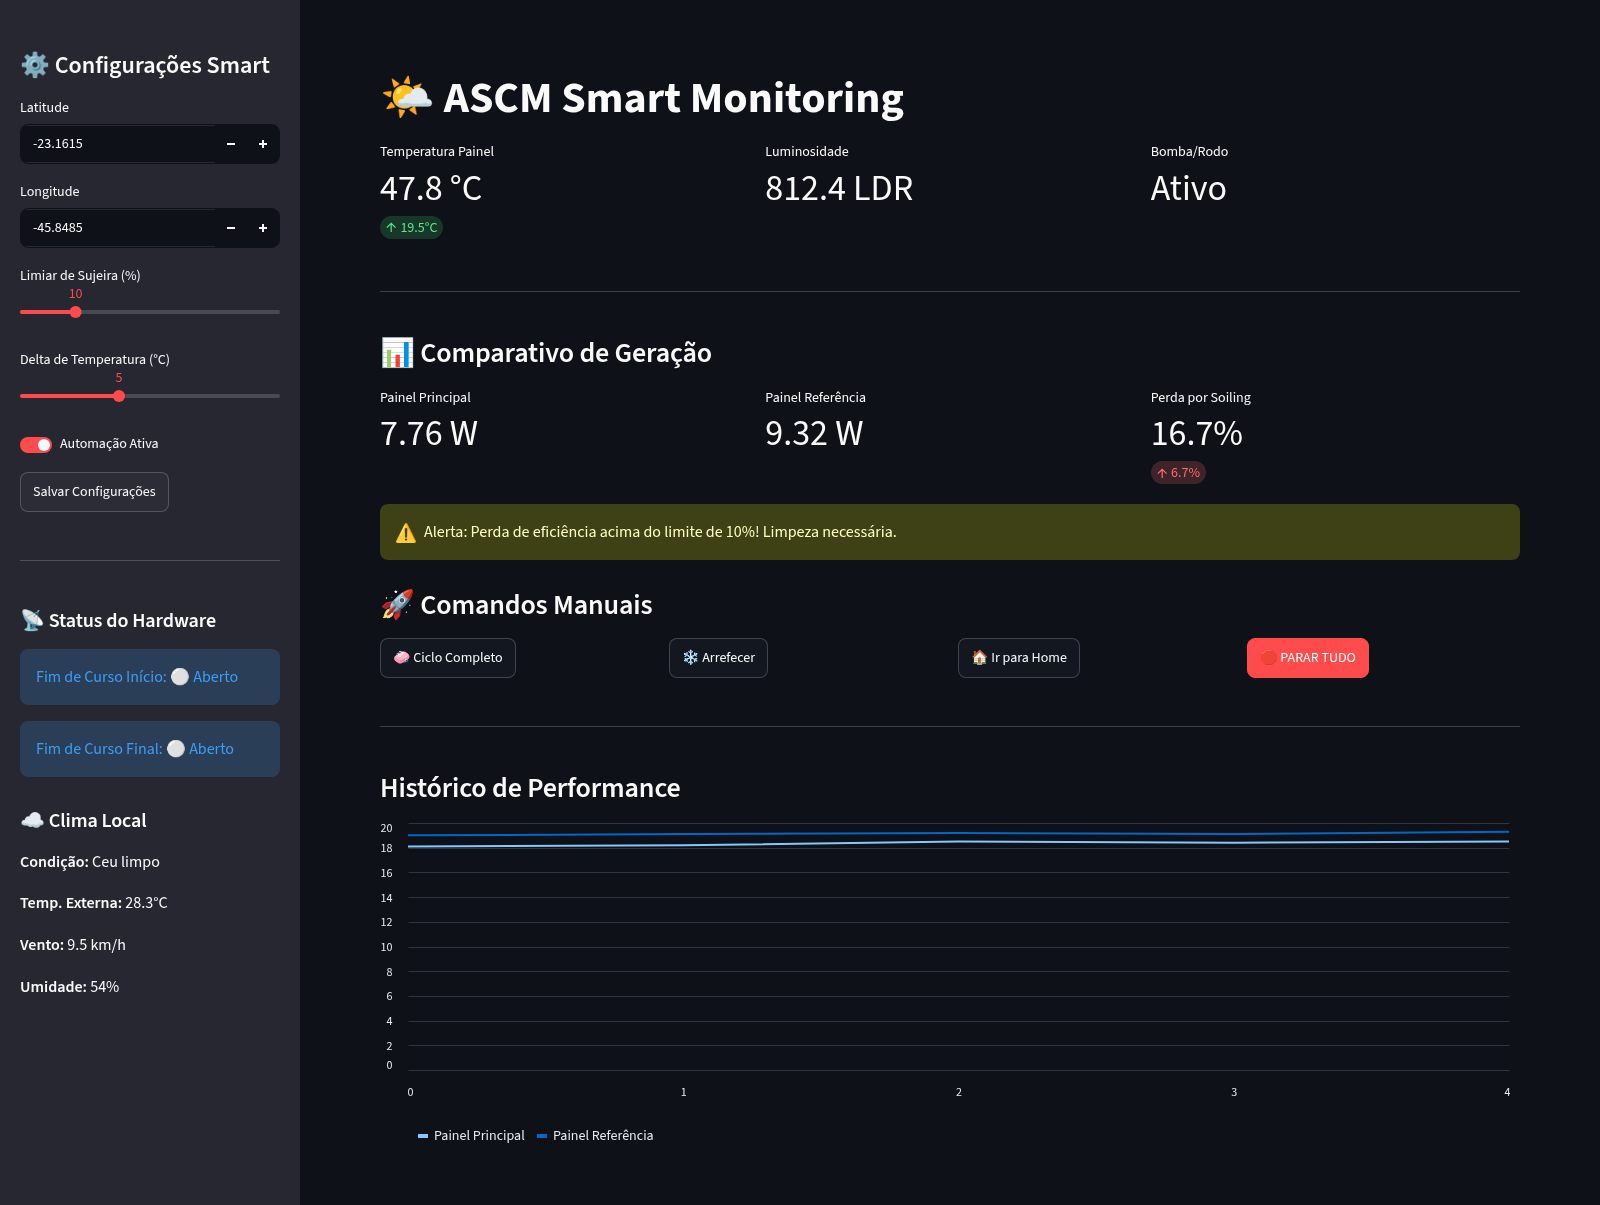
\includegraphics[width=\textwidth]{dashboard_streamlit.png}
    \caption{Dashboard Streamlit do ASCM renderizado com dados de exemplo (perda por soiling de 16,7\%, acima do limiar de 10\% configurado, disparando o alerta visual).}
    \label{fig:dashboard}
    \centerline{\small Fonte: Elaborado pelos autores.}
\end{figure}

O dashboard foi projetado para operar de forma resiliente: caso o backend esteja indisponível, as chamadas HTTP falham silenciosamente e a interface recorre a valores padrão neutros, evitando que uma falha de conexão com o Arduino derrube a experiência de monitoramento remoto.

\subsection{Estratégia do Laço de Controle Automatizado}
\label{sec:estrategia-controle}

A estratégia de automação funciona em ciclo contínuo em segundo plano e adota dois gatilhos paralelos e complementares:
\begin{enumerate}
    \item \textbf{Algoritmo de Resfriamento Térmico:} A temperatura da superfície do painel fotovoltaico ($T_{painel}$) é medida pelo termopar LM35 e comparada com a temperatura ambiente real ($T_{amb}$) retornada pelo serviço de meteorologia. O resfriamento é disparado se:
    \begin{equation}
        T_{painel} > T_{amb} + \Delta T_{lim}
    \end{equation}
    onde $\Delta T_{lim}$ é o diferencial limite definido no sistema (padrão de 5$^\circ$C). A bomba de água é acionada em modo de fluxo alto por um período programado até que a temperatura do painel se estabilize abaixo do limiar.
    \item \textbf{Algoritmo de Higienização de Sujeira:} A potência gerada pelo painel principal ($P_{main}$) e pelo painel de referência sujo ($P_{ref}$) são calculadas pelos respectivos sensores de potência INA219. A perda percentual por \textit{soiling} ($\Delta \eta$) é dada por:
    \begin{equation}
        \Delta \eta = \left( \frac{P_{ref} - P_{main}}{P_{ref}} \right) \times 100\%
    \end{equation}
    Se $\Delta \eta > \eta_{lim}$ (onde $\eta_{lim}$ é o limiar de sujeira tolerado, tipicamente 10\%) e a API de clima indicar que não há precipitação de chuva em andamento, o backend FastAPI invoca a tarefa assíncrona de ciclo de limpeza completo:
    \begin{itemize}
        \item Ativação da bomba d'água em fluxo baixo para molhar a poeira e amolecer o \textit{hard scale} por 2 segundos.
        \item Deslocamento do rodo mecânico na direção progressiva (\textit{forward}) com velocidade controlada via PWM até atingir a chave fim de curso final (\textit{limit\_end}).
        \item Breve pausa de 1 segundo e subsequente reversão do motor na direção contrária (\textit{backward}) até pressionar a chave fim de curso inicial (\textit{limit\_home}).
        \item Desligamento do motor e da bomba hidráulica, retornando o sistema ao monitoramento em malha fechada.
    \end{itemize}
\end{enumerate}

A lógica de funcionamento integrada de controle periódico, monitoramento de limites e acionamentos automáticos baseados nas decisões térmicas e de sujeira é apresentada no fluxograma de controle da Figura \ref{fig:fluxograma_controle}.

\begin{figure}[htbp]
    \centering
    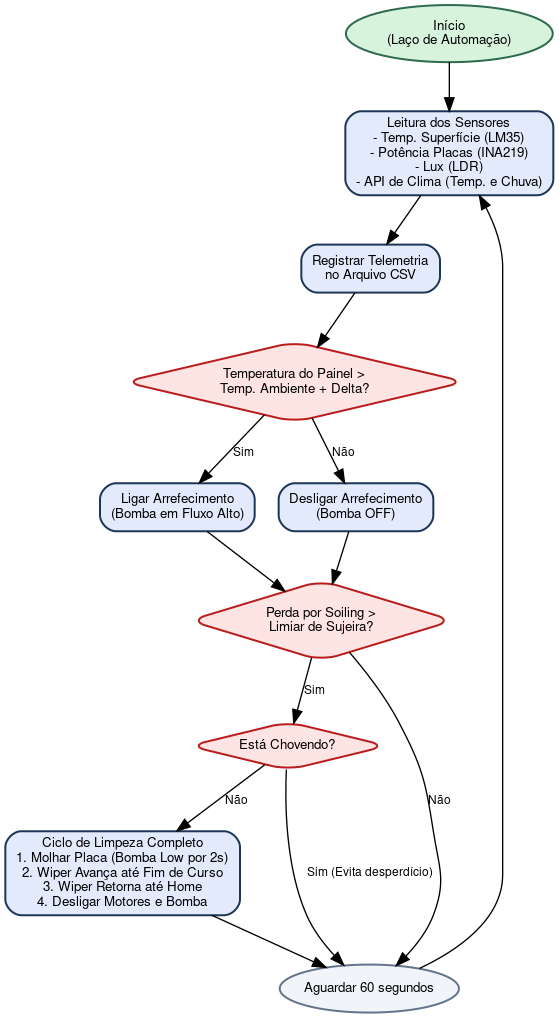
\includegraphics[width=0.55\textwidth]{fluxograma.png}
    \caption{Fluxograma do laço de controle de automação e de tomada de decisão do sistema ASCM.}
    \label{fig:fluxograma_controle}
    \centerline{\small Fonte: Elaborado pelos autores.}
\end{figure}

\subsection{Testes Automatizados de Software}

A camada de hardware (\texttt{HardwareManager}) possui suíte de testes unitários que substitui (\textit{mock}) a comunicação real via Telemetrix, permitindo validar a lógica de controle sem depender de um Arduino fisicamente conectado. Três classes de teste são cobertas: (i) controle correto de PWM da bomba para os níveis \texttt{high}/\texttt{low}/\texttt{off}; (ii) respeito às travas de fim de curso, verificando que o motor do rodo é impedido de avançar quando o sensor de fim de curso correspondente já foi acionado; e (iii) atualização correta do estado interno a partir dos \textit{callbacks} simulados de LDR e termopar. Essa abordagem permite integração contínua do firmware/backend sem exigir bancada de hardware físico disponível em todo ambiente de desenvolvimento.

\section{Resultados Preliminares e Metodologia de Ensaios}
\label{sec:resultados}

Esta seção descreve a validação inicial do software de controle e detalha a metodologia projetada para os futuros ensaios empíricos com o protótipo físico completo montado.

\subsection{Validação do Loop de Automação de Software}

Durante as simulações do software de controle, as rotinas de \textit{callback} do Telemetrix integradas à biblioteca FastAPI demonstraram latência inferior a 15 ms para detecção das chaves fim de curso, garantindo uma parada de emergência segura para os motores de movimentação linear do rodo. As leituras em barramento compartilhado dos sensores INA219 a frequências de amostragem de 1 Hz mostraram-se estáveis, com flutuações de corrente e tensão inferiores a 1,2\%, adequadas para o cálculo preciso do rendimento diferencial.

\subsection{Metodologia para Ensaio de Curto Prazo (Ambiente Controlado)}

Como validação preliminar do laço de automação antes do ensaio de campo de longo prazo, será conduzido um ensaio de curto prazo em ambiente controlado, com sujeira induzida e sob simulador de luz artificial, garantindo irradiância e temperatura estáveis. O procedimento seguirá as seguintes etapas:
\begin{enumerate}
    \item O painel de referência limpo ($P_{ref}$) e o painel principal do protótipo ($P_{main}$) serão instalados sob o simulador solar.
    \item No instante inicial ($t=0$ min), ambos os painéis estarão limpos para calibração de base ($P_{main} \approx P_{ref}$).
    \item Será induzida poeira artificial de forma controlada e progressiva sobre o painel principal, monitorando-se a queda de tensão e corrente elétrica geradas, a fim de levantar a curva de soiling diferencial ($\Delta \eta$).
    \item Ao ultrapassar o limiar programado ($\eta_{lim} = 10\%$), o laço de controle do ASCM disparará o ciclo automático de aspersão com raspagem mecânica do rodo sobre o painel principal, medindo-se a recuperação instantânea de sua potência elétrica.
\end{enumerate}

\subsection{Metodologia para Ensaio de Longo Prazo (Campo)}

O ensaio de campo, de longo prazo (30 dias) e sujeira natural, representa a validação definitiva do sistema em condições reais de operação, sendo complementar ao ensaio de curto prazo. O procedimento seguirá as seguintes etapas:
\begin{enumerate}
    \item Ambos os painéis (principal e referência) serão instalados externamente em suporte ajustável, expostos sob as mesmas condições de inclinação, orientação geográfica e sombreamento.
    \item No dia inicial ($t=0$), ambos os painéis serão limpos manualmente com água deionizada para garantir calibração inicial idêntica ($P_{main} \approx P_{ref}$).
    \item O painel de referência será mantido sob exposição ao acúmulo natural de poeira local por um período contínuo de 30 dias, sem passar por nenhum ciclo de limpeza automática.
    \item O painel principal passará pela automação do ASCM, disparando ciclos de limpeza sempre que a diferença de potência ultrapassar o limiar programado ($\eta_{lim} = 10\%$).
    \item Os parâmetros de geração (tensão, corrente, potência de pico e energia diária acumulada) serão registrados minuto a minuto para ambos os painéis, via o próprio \texttt{CSVLogger} do backend. A irradiância local relativa será monitorada via LDR.
\end{enumerate}

\subsection{Resultados Estimados do Ensaio de Curto Prazo}

A Tabela \ref{tab:ensaio_soiling} apresenta os dados estimados da atenuação de eficiência esperados durante o ensaio controlado sob luz artificial constante, ilustrando o padrão de perda de rendimento induzida e a posterior recuperação após a ativação do protótipo.

\begin{table}[htbp]
    \centering
    \caption{Dados estimados para o ensaio de curto prazo com sujidade induzida sob luz artificial.}
    \label{tab:ensaio_soiling}
    \begin{tabular}{cccccc}
    \toprule
    \textbf{Tempo (min)} & \textbf{Irradiância} & \textbf{$P_{main}$} & \textbf{$P_{ref}$} & \textbf{$\Delta \eta$} & \textbf{Status} \\
    \midrule
    0 (Inicial) & 1000 W/m$^2$ & 9,50 W & 9,50 W & 0,0\% & Calibrado (Limpo) \\
    10 & 1000 W/m$^2$ & 9,21 W & 9,50 W & 3,1\% & Operacional \\
    20 & 1000 W/m$^2$ & 8,84 W & 9,50 W & 6,9\% & Operacional \\
    30 & 1000 W/m$^2$ & 8,45 W & 9,50 W & 11,1\% & Limpeza Ativada \\
    32 (Pós-Limpeza) & 1000 W/m$^2$ & 9,48 W & 9,50 W & 0,2\% & Eficiência Recuperada \\
    \bottomrule
    \end{tabular}
\end{table}

\subsection{Ensaio de Arrefecimento e Ganho de Potência por Resfriamento}

Além do ensaio de sujidade, o termopar LM35 em conjunto com a bomba aspersora possibilitará a realização do ensaio térmico. Sob irradiância solar máxima no período do meio-dia (onde o painel atinge temperaturas elevadas superiores a 50$^\circ$C), o resfriamento evaporativo será acionado. Será mapeada a curva de queda de temperatura vs. o ganho de potência instantânea resultante. Os resultados esperados, embasados na literatura, preveem uma redução térmica estável de 5$^\circ$C a 10$^\circ$C na temperatura de operação das células, correspondendo a uma recuperação linear de potência entre 2,5\% e 6,0\% no instante de resfriamento.

\subsection{Discussão: Custos e Limitações}

O custo total de montagem do protótipo, considerando componentes eletrônicos COTS e material de impressão 3D em PLA, situa-se abaixo do custo de soluções industriais de limpeza robotizada, o que reforça a viabilidade da proposta para instalações de pequeno porte. Entre as limitações identificadas até o presente estágio do projeto, destacam-se: (i) a dependência de conexão serial contínua entre o Arduino e o computador hospedeiro, o que restringe o alcance físico da instalação sem o uso de conversores serial-Ethernet/Wi-Fi; (ii) o uso de PLA no protótipo de teste, material que não é recomendado para exposição solar contínua de longo prazo devido à sua temperatura de amolecimento relativamente baixa, o que motiva a recomendação de PETG ou ABS em versões de campo; e (iii) a dependência de uma API meteorológica externa (Open-Meteo) para a decisão de suspensão de limpeza em dias chuvosos, o que introduz uma dependência de conectividade à internet no local de instalação.

\section{Considerações Finais}
\label{sec:conclusao}

O protótipo do ASCM projetado demonstrou-se viável sob o aspecto de desenvolvimento de software e integração de hardware de baixo custo, orçando um custo total de montagem inferior ao de soluções industriais. O uso do protocolo Telemetrix permitiu a criação de um laço de automação flexível e centralizado no computador hospedeiro via FastAPI e Streamlit, com uma API REST documentada e testável independentemente do hardware físico, e um dashboard capaz de operar de forma resiliente mesmo diante de falhas de conexão.

Os próximos passos deste trabalho consistem no término do acoplamento mecânico estrutural do rodo impresso em 3D no painel solar físico e no início imediato dos ensaios de degradação por sujidade de 30 dias e dos testes térmicos. Espera-se, com esses testes, validar a eficácia prática da aspersão com raspagem mecânica na remoção de poeira consolidada (\textit{hard scale}) e quantificar o ganho líquido anual de geração elétrica proporcionado pelo sistema.

\section*{Contribuições dos Autores}

L. E. contribuiu com: Concepção, Metodologia, Software, Investigação e Escrita – rascunho original. P. R. contribuiu com: Metodologia, Software, Recursos, Investigação, Visualização e Escrita – rascunho original. C. K. contribuiu com: Metodologia, Recursos, Investigação e Visualização. V. D. G. contribuiu com: Supervisão e Escrita – revisão e edição.

\section*{Agradecimentos}

Os autores agradecem ao Instituto Federal de Educação, Ciência e Tecnologia de São Paulo (IFSP) Câmpus São José dos Campos pelo apoio estrutural e pedagógico para o desenvolvimento deste projeto de iniciação tecnológica.

\bibliographystyle{plain}
\bibliography{CONICT/bibliografia}

\end{document}
